% OrbitCraft 2D — Tutorial (English version). Compile with XeLaTeX (see build.ps1).
\documentclass[11pt]{article}
\newcommand{\tr}[2]{#2}
\usepackage[english]{babel}
% Shared style for the OrbitCraft 2D internal tutorial (Vietnamese + English).
% Compile with XeLaTeX (see build.ps1). Each main file defines \tr before \input-ing this:
%   \newcommand{\tr}[2]{#1}  % Vietnamese  |  \newcommand{\tr}[2]{#2}  % English

\usepackage[a4paper, margin=2cm, headheight=14pt]{geometry}
\usepackage{fontspec}
\setmainfont{Cambria}
\setsansfont{Calibri}
\setmonofont{Consolas}[Scale=0.92]
\newfontfamily\symfont{Segoe UI Symbol}

\usepackage{amsmath}
\usepackage{xcolor}
\usepackage{graphicx}
\usepackage{float}
\usepackage{tabularx, booktabs, array}
\usepackage{enumitem}
\usepackage{fancyhdr}
\usepackage{titlesec}
\usepackage[most]{tcolorbox}
\usepackage{tikz}
\usetikzlibrary{positioning, arrows.meta, shapes.geometric, fit, backgrounds, calc}
\usepackage[hidelinks]{hyperref}
\usepackage{xurl}

% ---------- colours (match the game UI) ----------
\definecolor{accent}{HTML}{1F6FB2}
\definecolor{accentlight}{HTML}{E8F1FA}
\definecolor{ink}{HTML}{1E2433}
\definecolor{muted}{HTML}{5B6478}
\definecolor{okc}{HTML}{2A8A3C}
\definecolor{warnc}{HTML}{C98A00}
\definecolor{failc}{HTML}{C0392B}
\definecolor{rule}{HTML}{C9D3E3}
\color{ink}

% ---------- layout ----------
\setlength{\parindent}{0pt}
\setlength{\parskip}{5pt}
\linespread{1.08}
\setlist{itemsep=2pt, topsep=3pt, leftmargin=*}
\renewcommand{\arraystretch}{1.25}

\titleformat{\section}{\sffamily\LARGE\bfseries\color{accent}}{\thesection.}{0.5em}{}[{\color{accent}\titlerule[1pt]}]
\titleformat{\subsection}{\sffamily\Large\bfseries\color{ink}}{\thesubsection}{0.5em}{}
\titleformat{\subsubsection}{\sffamily\large\bfseries\color{muted}}{\thesubsubsection}{0.5em}{}
\titlespacing*{\section}{0pt}{16pt}{8pt}
\titlespacing*{\subsection}{0pt}{12pt}{4pt}
\titlespacing*{\subsubsection}{0pt}{10pt}{3pt}
\renewcommand{\thesection}{\Roman{section}}
\renewcommand{\thesubsection}{\arabic{subsection}.}
\renewcommand{\thesubsubsection}{\arabic{subsection}.\arabic{subsubsection}}

\pagestyle{fancy}
\fancyhf{}
\fancyhead[L]{\sffamily\small\color{muted} OrbitCraft 2D --- \tr{Hướng dẫn}{Tutorial}}
\fancyhead[R]{\sffamily\small\color{muted} \tr{Tài liệu nội bộ}{Internal document}}
\fancyfoot[C]{\sffamily\small\color{muted}\thepage}
\renewcommand{\headrulewidth}{0.4pt}
\renewcommand{\headrule}{{\color{rule}\hrule width\headwidth height\headrulewidth}}

% ---------- inline helpers ----------
\newcommand{\code}[1]{\texttt{\detokenize{#1}}}
\newcommand{\kbd}[1]{\tikz[baseline=(k.base)]\node[draw=muted, rounded corners=1.5pt, inner xsep=2.5pt, inner ysep=1.2pt, fill=accentlight, font=\ttfamily\footnotesize](k){#1};}
\newcommand{\starsym}{{\symfont ★}}
\newcommand{\stars}[1]{\leavevmode{\color{warnc}\symfont\foreach \i in {1,...,#1}{★}}}
\newcommand{\outcome}[1]{{\ttfamily\small\color{failc}\detokenize{#1}}}
\newcommand{\dv}{$\Delta v$}

% ---------- tables ----------
\newcolumntype{L}{>{\raggedright\arraybackslash}X}
\newcolumntype{P}[1]{>{\raggedright\arraybackslash}p{#1}}
\newcommand{\thead}[1]{\sffamily\bfseries\small #1}
\newenvironment{dtable}[1]
  {\par\small\noindent\tabularx{\linewidth}{#1}\toprule}
  {\bottomrule\endtabularx\par}

% ---------- callout boxes ----------
\newtcolorbox{tipbox}[1][]{enhanced, breakable, colback=accentlight, colframe=accent, boxrule=0.6pt,
  arc=2pt, left=8pt, right=8pt, top=5pt, bottom=5pt, fonttitle=\sffamily\bfseries, #1}
\newtcolorbox{warnbox}[1][]{enhanced, breakable, colback=warnc!8, colframe=warnc, boxrule=0.6pt,
  arc=2pt, left=8pt, right=8pt, top=5pt, bottom=5pt, fonttitle=\sffamily\bfseries, #1}
\newtcolorbox{sourcebox}[1]{enhanced, colback=white, colframe=rule, boxrule=0.5pt, arc=2pt,
  left=8pt, right=8pt, top=4pt, bottom=4pt, title={#1}, coltitle=ink, colbacktitle=accentlight,
  fonttitle=\sffamily\bfseries, attach boxed title to top left={yshift=-2mm, xshift=4mm},
  boxed title style={colframe=rule, boxrule=0.5pt, arc=2pt}}

% ---------- figure frame ----------
% \begin{diagram}{caption}{label} ... \end{diagram}
\newenvironment{diagram}[2]
  {\begin{figure}[H]\centering\def\diagramcaption{#1}\def\diagramlabel{#2}%
   \begin{tcolorbox}[colback=white, colframe=rule, boxrule=0.5pt, arc=2pt, width=\linewidth, halign=center]}
  {\end{tcolorbox}\caption{\diagramcaption}\label{\diagramlabel}\end{figure}}

\usepackage{caption}
\captionsetup{font={small,sf}, labelfont={bf,color=accent}}

% ---------- TikZ styles shared by all diagrams ----------
\tikzset{
  ocbase/.style={rectangle, rounded corners=3pt, align=center, font=\sffamily\small, inner sep=5pt, thick},
  ocstep/.style={ocbase, draw=accent, fill=accentlight, minimum width=58mm, minimum height=11mm},
  ocaux/.style={ocbase, draw=muted, fill=white, dashed, minimum width=40mm, minimum height=11mm},
  ocgood/.style={ocbase, draw=okc, fill=okc!10, minimum width=58mm, minimum height=10mm},
  ocdecision/.style={diamond, aspect=2.6, draw=warnc, fill=warnc!10, thick, align=center, font=\sffamily\small\bfseries, inner sep=1.5pt},
  occheck/.style={ocbase, draw=accent, fill=white, minimum width=50mm, minimum height=8mm, inner sep=3pt},
  ocfail/.style={rectangle, rounded corners=2pt, draw=failc, fill=failc!8, font=\ttfamily\footnotesize, text=failc, minimum width=38mm, minimum height=7mm},
  ocwin/.style={rectangle, rounded corners=8pt, draw=okc, fill=okc!15, thick, font=\sffamily\small\bfseries, text=okc, minimum width=50mm, minimum height=8mm},
  ocmodule/.style={ocbase, draw=accent, fill=white, minimum width=34mm, minimum height=10mm, inner sep=3pt},
  ocarr/.style={-{Stealth[length=2.6mm]}, thick, draw=ink},
  ocokarr/.style={-{Stealth[length=2.4mm]}, thick, draw=okc},
  ocfailarr/.style={-{Stealth[length=2.2mm]}, dashed, draw=failc},
  oclbl/.style={font=\sffamily\scriptsize, fill=white, inner sep=1.5pt, text=muted, align=center},
  ocgroup/.style={rectangle, rounded corners=5pt, draw=rule, fill=#1, inner sep=7pt},
  ocgroup/.default=accentlight!45,
  ocgrouplabel/.style={font=\sffamily\footnotesize\bfseries, text=accent},
}


\hypersetup{pdftitle={OrbitCraft 2D - Tutorial}, pdfsubject={NASA Space Apps Challenge 2026}}

\begin{document}

% ------------------------------------------------------------ title block (no cover page)
{\sffamily
{\fontsize{26}{30}\selectfont\bfseries\color{accent} OrbitCraft 2D}\\[2pt]
{\Large\color{ink} Project overview and how to play}\\[6pt]
{\small\color{muted} Internal team document · \emph{Space Mission Design Game} challenge --- NASA Space Apps Challenge 2026 · Updated \today}\par}
\vspace{4pt}{\color{accent}\rule{\linewidth}{1.2pt}}

\begin{tipbox}
\textbf{Run the game:} open a terminal in the project folder, run \code{npm install} (first time only) then \code{npm run dev}; the browser opens \url{http://localhost:8080}. \quad
\textbf{Run the tests:} \code{npm test}.
\end{tipbox}

{\small\setcounter{tocdepth}{2}\tableofcontents}

% ============================================================ I
\section{Project overview}

\subsection{The problem}

Designing a space mission is a problem of \textbf{trade-offs}: every engineering choice sets off a chain of consequences.

\begin{itemize}
  \item Add one more science instrument and the spacecraft gets heavier, the rocket loses delta-v (\dv), and the spacecraft needs more power.
  \item Add solar panels to get enough power and you add mass and cost.
  \item Drop the tail fins to save weight and the rocket becomes unstable and tumbles right after leaving the pad.
\end{itemize}

The challenge asks for a game in which players \textbf{design, manage and simulate} a complete mission themselves. Players must balance 9 factors: mission goals, spacecraft design, science instruments, launch vehicle, budget, power, mass, communications and orbit.

Professional tools such as GMAT are too complex for students and beginners. On the other hand, many ``space'' games are just quizzes or pre-made animations: players see \textbf{success / failure} but never learn \textbf{why}.

\subsection{The solution}

\textbf{OrbitCraft 2D} is a lightweight 2D pixel-art web game that runs directly in the browser. Real physics decides every outcome, and the game always explains the cause.

\begin{dtable}{P{38mm}L}
\thead{Key idea} & \thead{How the game shows it} \\ \midrule
\textbf{Instant cause and effect} & Every time a part changes, the data panel and the \textbf{CG / CP} markers on the rocket update immediately. Players know in advance what will break. \\
\textbf{Real physics} & Tsiolkovsky rocket equation for each stage, thrust-to-weight ratio, static stability margin from TIR-33, power balance through the orbit's eclipse, radio range and bandwidth. \\
\textbf{Failure post-mortem} & After every flight, the report shows the \textbf{root cause}, the \textbf{parts at fault} and \textbf{how to fix it}. Press \emph{Fix in Workshop} to go back; the faulty parts flash red. \\
\textbf{12 different outcomes} & Stuck on the pad, tumble, not enough \dv, stranded in parking orbit, dead bus, thermal failure, loss of signal, data bottleneck, science shortfall, over budget, invalid design, success. \\
\textbf{NASA data} & Small spacecraft classes, launcher types and mission scenarios come from NASA documents. Every part names its source (see Part~III). \\
\end{dtable}

\subsection{Main workflow}

\subsubsection{Game loop}

Players move through 4 screens in order (Figure~\ref{fig:loop}). In the workshop, every change re-runs the simulation instantly, so players can see which check will fail before they press launch.

\begin{diagram}{Main game loop: from choosing a mission to the post-mortem report and back to fix the design.}{fig:loop}
% Figure: main game loop (Mission Briefing -> Workshop -> Launch -> Report -> back).
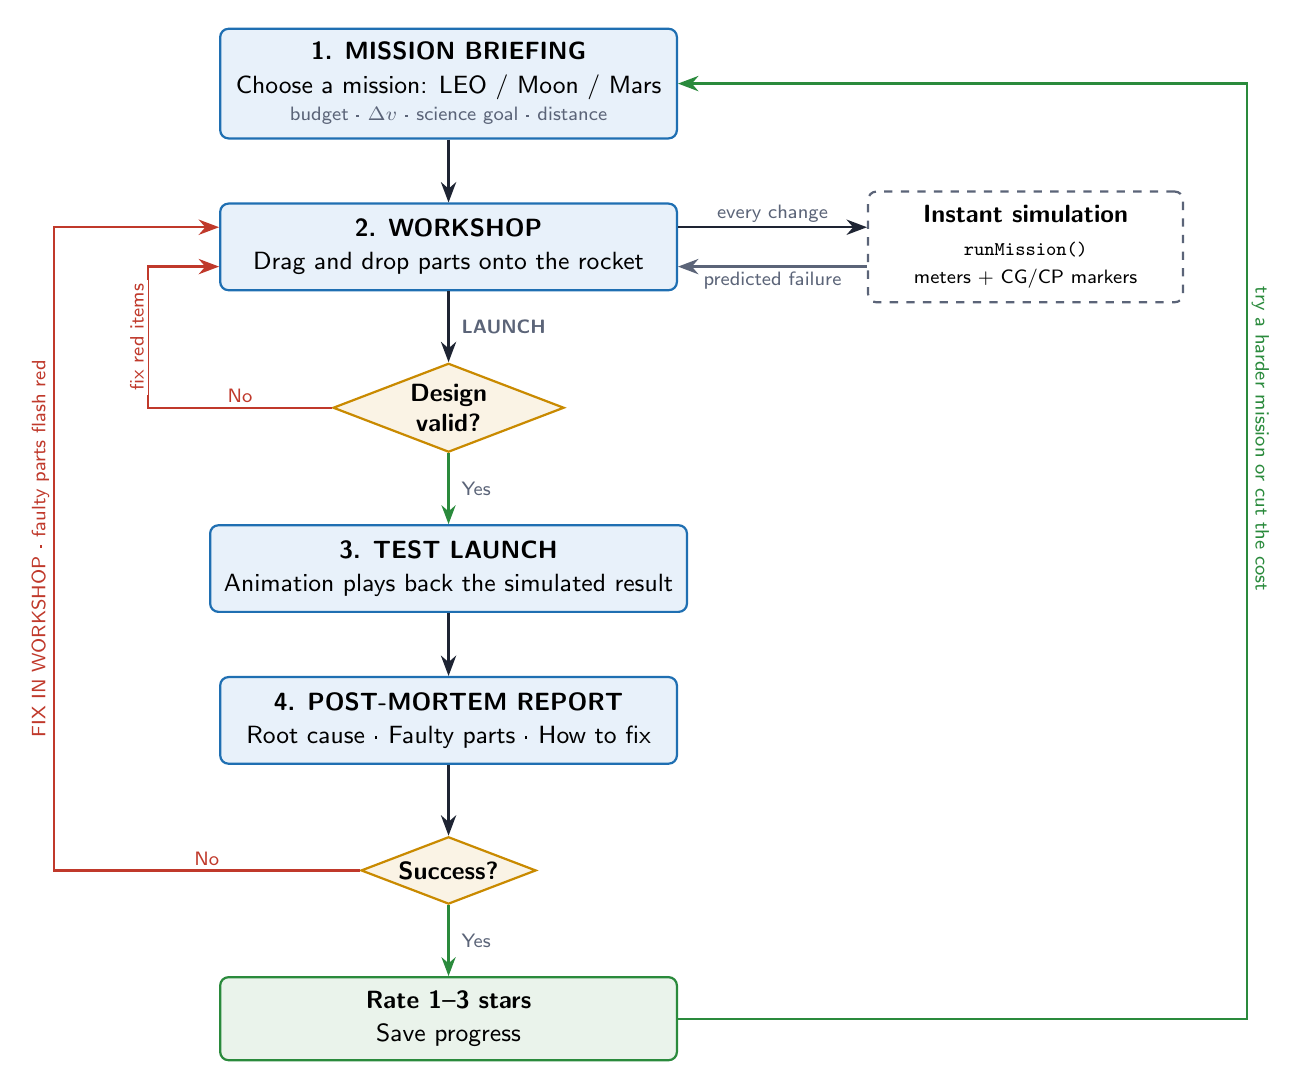
\begin{tikzpicture}[node distance=8mm and 14mm]
  \node[ocstep] (A) {\textbf{1. MISSION BRIEFING}\\[1pt]
    \tr{Chọn nhiệm vụ: LEO / Mặt Trăng / Sao Hỏa}{Choose a mission: LEO / Moon / Mars}\\[-1pt]
    {\scriptsize\color{muted}\tr{ngân sách · $\Delta v$ · mục tiêu khoa học · khoảng cách}{budget · $\Delta v$ · science goal · distance}}};
  \node[ocstep, below=of A] (B) {\textbf{2. \tr{XƯỞNG LẮP RÁP}{WORKSHOP}}\\[1pt]
    \tr{Kéo-thả linh kiện lên tên lửa}{Drag and drop parts onto the rocket}};
  \node[ocaux, right=24mm of B] (C) {\textbf{\tr{Mô phỏng tức thì}{Instant simulation}}\\[1pt]
    {\scriptsize\code{runMission()}}\\[-1pt]{\scriptsize \tr{thanh đo + mốc CG/CP}{meters + CG/CP markers}}};
  \node[ocdecision, below=9mm of B] (D) {\tr{Thiết kế\\hợp lệ?}{Design\\valid?}};
  \node[ocstep, below=9mm of D] (E) {\textbf{3. \tr{PHÓNG THỬ NGHIỆM}{TEST LAUNCH}}\\[1pt]
    \tr{Hoạt ảnh phát lại kết quả mô phỏng}{Animation plays back the simulated result}};
  \node[ocstep, below=of E] (F) {\textbf{4. \tr{BÁO CÁO KHÁM NGHIỆM}{POST-MORTEM REPORT}}\\[1pt]
    \tr{Nguyên nhân · Linh kiện lỗi · Cách sửa}{Root cause · Faulty parts · How to fix}};
  \node[ocdecision, below=9mm of F] (G) {\tr{Thành\\công?}{Success?}};
  \node[ocgood, below=9mm of G] (H) {\textbf{\tr{Chấm 1--3 sao}{Rate 1--3 stars}}\\[1pt]
    \tr{Lưu thành tích}{Save progress}};

  % main spine
  \draw[ocarr] (A) -- (B);
  \draw[ocarr] (B) -- node[oclbl, right=1mm]{\textbf{LAUNCH}} (D);
  \draw[ocokarr] (D) -- node[oclbl, right=1mm]{\tr{Có}{Yes}} (E);
  \draw[ocarr] (E) -- (F);
  \draw[ocarr] (F) -- (G);
  \draw[ocokarr] (G) -- node[oclbl, right=1mm]{\tr{Có}{Yes}} (H);

  % live simulation loop
  \draw[ocarr] ([yshift=2.5mm]B.east) -- node[oclbl, above]{\tr{mỗi thay đổi}{every change}} ([yshift=2.5mm]C.west);
  \draw[ocarr, draw=muted] ([yshift=-2.5mm]C.west) -- node[oclbl, below]{\tr{dự đoán lỗi}{predicted failure}} ([yshift=-2.5mm]B.east);

  % left-hand loops back to the workshop
  \coordinate (L1) at ($(B.west)+(-9mm,0)$);
  \coordinate (L2) at ($(B.west)+(-21mm,0)$);
  \draw[ocarr, draw=failc] (D.west) -- node[oclbl, above, text=failc]{\tr{Không}{No}} (D.west -| L1)
        |- ([yshift=-2.5mm]B.west);
  \node[oclbl, rotate=90, anchor=south, text=failc] at ($(D.west -| L1)!0.5!([yshift=-2.5mm]B.west -| L1)$) {\tr{sửa lỗi đỏ}{fix red items}};
  \draw[ocarr, draw=failc] (G.west) -- node[oclbl, above, text=failc]{\tr{Không}{No}} (G.west -| L2)
        |- ([yshift=2.5mm]B.west);
  \node[oclbl, rotate=90, anchor=south, text=failc] at ($(G.west -| L2)!0.5!([yshift=2.5mm]B.west -| L2)$)
        {FIX IN WORKSHOP · \tr{linh kiện lỗi nhấp nháy đỏ}{faulty parts flash red}};

  % right-hand loop: next mission
  \coordinate (R) at ($(C.east)+(8mm,0)$);
  \draw[ocarr, draw=okc] (H.east) -- (H.east -| R) |- (A.east);
  \node[oclbl, rotate=-90, anchor=south, text=okc] at ($(H.east -| R)!0.62!(A.east -| R)$)
        {\tr{thử nhiệm vụ khó hơn hoặc tối ưu chi phí}{try a harder mission or cut the cost}};
\end{tikzpicture}

\end{diagram}

\subsubsection{Launch check sequence}

The simulator (\code{src/core/simulate.js}) runs 11 checks \textbf{in flight order} (Figure~\ref{fig:checks}). The \textbf{first failing check} is the root cause. Later checks are still evaluated and shown in the report as \emph{(predicted)}, so players can fix everything in one go. The LEO mission has no transfer step.

\begin{diagram}{Check sequence in flight order, and the outcome produced when each check fails.}{fig:checks}
% Figure: the simulator's check sequence, in flight order, with the outcome each failure produces.
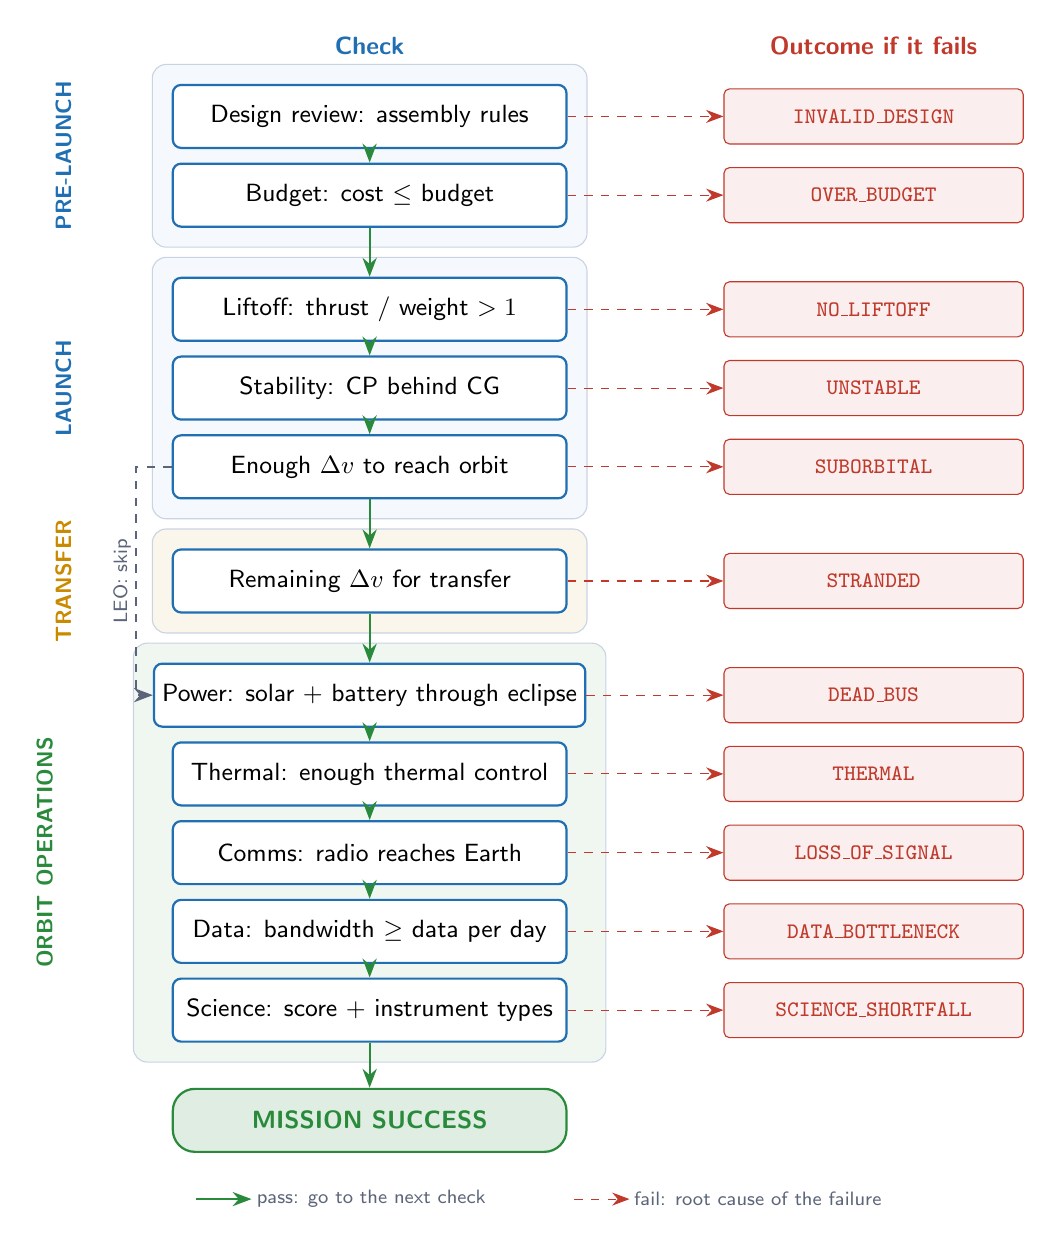
\begin{tikzpicture}[x=1cm, y=1cm]
  % ----- checks (centre column) and outcomes (right column)
  \newcommand{\chk}[5]{% name, y, title, outcome code, outcome label
    \node[occheck] (#1) at (0,#2) {#3};
    \node[ocfail] (#1f) at (6.4,#2) {#4};
    \draw[ocfailarr] (#1.east) -- (#1f.west);
  }
  \chk{c1}{0}{\tr{Design review: lắp đúng quy tắc}{Design review: assembly rules}}{INVALID\_DESIGN}{}
  \chk{c2}{-1.0}{\tr{Budget: chi phí $\le$ ngân sách}{Budget: cost $\le$ budget}}{OVER\_BUDGET}{}
  \chk{c3}{-2.45}{\tr{Liftoff: lực đẩy / trọng lượng $> 1$}{Liftoff: thrust / weight $> 1$}}{NO\_LIFTOFF}{}
  \chk{c4}{-3.45}{\tr{Stability: CP nằm sau CG}{Stability: CP behind CG}}{UNSTABLE}{}
  \chk{c5}{-4.45}{\tr{$\Delta v$ đủ để vào quỹ đạo}{Enough $\Delta v$ to reach orbit}}{SUBORBITAL}{}
  \chk{c6}{-5.9}{\tr{$\Delta v$ còn lại đủ để chuyển quỹ đạo}{Remaining $\Delta v$ for transfer}}{STRANDED}{}
  \chk{c7}{-7.35}{\tr{Power: điện mặt trời + pin qua vùng tối}{Power: solar + battery through eclipse}}{DEAD\_BUS}{}
  \chk{c8}{-8.35}{\tr{Thermal: đủ mức tản nhiệt}{Thermal: enough thermal control}}{THERMAL}{}
  \chk{c9}{-9.35}{\tr{Comms: radio đủ tầm tới Trái Đất}{Comms: radio reaches Earth}}{LOSS\_OF\_SIGNAL}{}
  \chk{c10}{-10.35}{\tr{Data: băng thông $\ge$ dữ liệu/ngày}{Data: bandwidth $\ge$ data per day}}{DATA\_BOTTLENECK}{}
  \chk{c11}{-11.35}{\tr{Science: đủ điểm + đủ loại thiết bị}{Science: score + instrument types}}{SCIENCE\_SHORTFALL}{}
  \node[ocwin] (ok) at (0,-12.75) {MISSION SUCCESS};

  % ----- pass arrows down the spine
  \foreach \a/\b in {c1/c2, c2/c3, c3/c4, c4/c5, c5/c6, c6/c7, c7/c8, c8/c9, c9/c10, c10/c11, c11/ok}
    \draw[ocokarr] (\a.south) -- (\b.north);

  % ----- LEO has no transfer: bypass on the left
  \draw[ocokarr, dashed, draw=muted] (c5.west) -- ++(-0.45,0) |- (c7.west)
     node[pos=0.25, oclbl, rotate=90, anchor=south, fill=white] {\tr{LEO: bỏ qua}{LEO: skip}};

  % ----- phase groups
  \begin{scope}[on background layer]
    \node[ocgroup, fit=(c1)(c2)] (g1) {};
    \node[ocgroup, fit=(c3)(c5)] (g2) {};
    \node[ocgroup=warnc!8, fit=(c6)] (g3) {};
    \node[ocgroup=okc!7, fit=(c7)(c11)] (g4) {};
  \end{scope}
  \node[ocgrouplabel, rotate=90, anchor=south] at ($(g1.west)+(-0.9,0)$) {\tr{TRƯỚC PHÓNG}{PRE-LAUNCH}};
  \node[ocgrouplabel, rotate=90, anchor=south] at ($(g2.west)+(-0.9,0)$) {\tr{PHÓNG}{LAUNCH}};
  \node[ocgrouplabel, rotate=90, anchor=south, text=warnc] at ($(g3.west)+(-0.9,0)$) {\tr{CHUYỂN}{TRANSFER}};
  \node[ocgrouplabel, rotate=90, anchor=south, text=okc] at ($(g4.west)+(-0.9,0)$) {\tr{VẬN HÀNH TRÊN QUỸ ĐẠO}{ORBIT OPERATIONS}};

  % ----- column headers + legend
  \node[font=\sffamily\small\bfseries, text=accent] at (0,0.9) {\tr{Bước kiểm tra}{Check}};
  \node[font=\sffamily\small\bfseries, text=failc] at (6.4,0.9) {\tr{Kết quả nếu hỏng}{Outcome if it fails}};
  \draw[ocokarr] (-2.2,-13.75) -- ++(0.7,0) node[right, oclbl, fill=none]{\tr{đạt: sang bước tiếp theo}{pass: go to the next check}};
  \draw[ocfailarr] (2.6,-13.75) -- ++(0.7,0) node[right, oclbl, fill=none]{\tr{hỏng: nguyên nhân gốc của thất bại}{fail: root cause of the failure}};
\end{tikzpicture}

\end{diagram}

\subsubsection{Code architecture}

The logic is fully separated from the display (Figure~\ref{fig:arch}). All of the physics lives in \code{src/core} as pure functions with no Phaser dependency, so it is covered by automated Node tests (\code{npm test}, 123 tests). The scenes only read the simulation result to display it, so the animation always matches the report.

\begin{diagram}{Code architecture: data $\to$ pure logic $\to$ display.}{fig:arch}
% Figure: code architecture (data -> pure logic -> display).
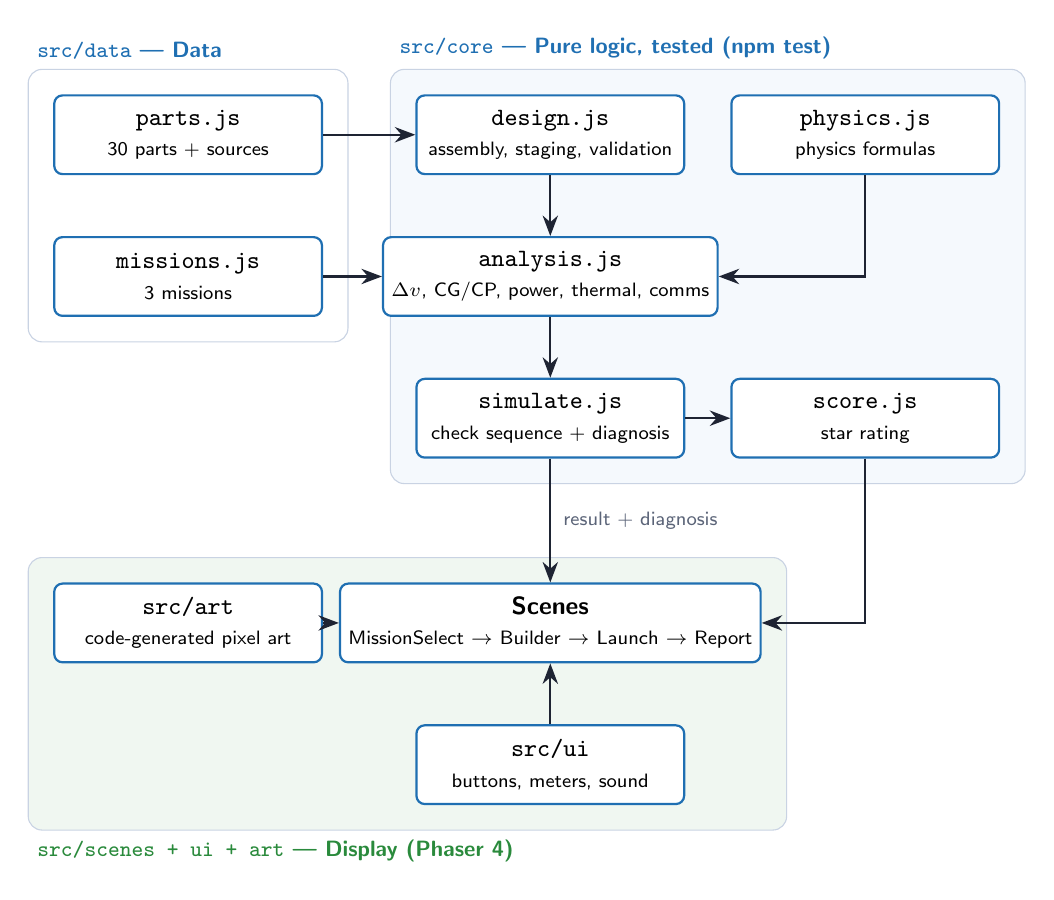
\begin{tikzpicture}[x=1cm, y=1cm]
  % data
  \node[ocmodule] (parts) at (0,1.2) {\code{parts.js}\\{\scriptsize\tr{30 linh kiện + nguồn}{30 parts + sources}}};
  \node[ocmodule] (missions) at (0,-0.6) {\code{missions.js}\\{\scriptsize\tr{3 nhiệm vụ}{3 missions}}};
  % core
  \node[ocmodule] (design) at (4.6,1.2) {\code{design.js}\\{\scriptsize\tr{lắp ráp, chia tầng, kiểm lỗi}{assembly, staging, validation}}};
  \node[ocmodule] (physics) at (8.6,1.2) {\code{physics.js}\\{\scriptsize\tr{công thức vật lý}{physics formulas}}};
  \node[ocmodule] (analysis) at (4.6,-0.6) {\code{analysis.js}\\{\scriptsize $\Delta v$, CG/CP, \tr{điện, nhiệt, liên lạc}{power, thermal, comms}}};
  \node[ocmodule] (simulate) at (4.6,-2.4) {\code{simulate.js}\\{\scriptsize\tr{chuỗi kiểm tra + chẩn đoán}{check sequence + diagnosis}}};
  \node[ocmodule] (score) at (8.6,-2.4) {\code{score.js}\\{\scriptsize\tr{chấm sao}{star rating}}};
  % view
  \node[ocmodule, minimum width=36mm] (scenes) at (4.6,-5.0) {\textbf{\tr{Các màn hình}{Scenes}}\\{\scriptsize MissionSelect $\to$ Builder $\to$ Launch $\to$ Report}};
  \node[ocmodule] (art) at (0,-5.0) {\code{src/art}\\{\scriptsize\tr{pixel art sinh bằng code}{code-generated pixel art}}};
  \node[ocmodule] (ui) at (4.6,-6.8) {\code{src/ui}\\{\scriptsize\tr{nút, thanh đo, âm thanh}{buttons, meters, sound}}};

  \begin{scope}[on background layer]
    \node[ocgroup=white, fit=(parts)(missions), inner sep=9pt] (gd) {};
    \node[ocgroup, fit=(design)(physics)(score)(simulate), inner sep=9pt] (gc) {};
    \node[ocgroup=okc!7, fit=(art)(scenes)(ui), inner sep=9pt] (gv) {};
  \end{scope}
  \node[ocgrouplabel, anchor=south west] at (gd.north west) {\code{src/data} --- \tr{Dữ liệu}{Data}};
  \node[ocgrouplabel, anchor=south west] at (gc.north west) {\code{src/core} --- \tr{Logic thuần, có test (npm test)}{Pure logic, tested (npm test)}};
  \node[ocgrouplabel, anchor=north west, text=okc] at (gv.south west) {\code{src/scenes + ui + art} --- \tr{Hiển thị (Phaser 4)}{Display (Phaser 4)}};

  \draw[ocarr] (parts) -- (design);
  \draw[ocarr] (missions) -- (analysis);
  \draw[ocarr] (physics.south) |- (analysis.east);
  \draw[ocarr] (design) -- (analysis);
  \draw[ocarr] (analysis) -- (simulate);
  \draw[ocarr] (simulate) -- (score);
  \draw[ocarr] (simulate) -- node[oclbl, right=1mm]{\tr{kết quả + chẩn đoán}{result + diagnosis}} (scenes);
  \draw[ocarr] (score.south) |- (scenes.east);
  \draw[ocarr] (art) -- (scenes);
  \draw[ocarr] (ui) -- (scenes);
\end{tikzpicture}

\end{diagram}

% ============================================================ II
\clearpage
\section{How to play}

\subsection{Choose a mission}

\begin{dtable}{P{33mm}P{24mm}P{13mm}P{17mm}L}
\thead{Mission} & \thead{Destination} & \thead{Budget} & \thead{\dv{} needed} & \thead{Science goal · Main challenge} \\ \midrule
\stars{1}~\textbf{Eyes on Earth} & Low Earth Orbit, 500\,km & \$25M & 9,400\,m/s & Score $\ge 2$, needs \emph{imaging}. Getting started: aerodynamic stability. \\
\stars{2}~\textbf{Lunar Prospector Jr.} & Low Lunar Orbit, 100\,km & \$40M & 13,400\,m/s & Score $\ge 4$, needs \emph{spectrometer}. Communicating across 384,400\,km. \\
\stars{3}~\textbf{Red Planet Scout} & Low Mars Orbit, 400\,km & \$70M & 15,100\,m/s & Score $\ge 6$, needs \emph{imaging} + \emph{spectrometer}. Weak sunlight (43\%), Earth is very far. \\
\end{dtable}

Click a mission card or press \kbd{1} \kbd{2} \kbd{3}. Each mission opens with a \textbf{starter design that has exactly one flaw} for you to find and fix.

\subsection{Build in the workshop}

The workshop has 3 columns:

\begin{dtable}{P{42mm}L}
\thead{Area} & \thead{What it does} \\ \midrule
\textbf{PARTS BIN} (left) & 11 part categories. Hover a part to see its specs and NASA source. \\
\textbf{BLUEPRINT} (centre) & The rocket on its launch pad. On the left: the stages (S1, S2, \dots) with their \dv. On the right: the \textbf{CG} (yellow) and \textbf{CP} (orange) markers and the stability margin. \\
\textbf{LIVE ENGINEERING DATA} (right) & One meter per check. {\color{okc}Green} = pass, {\color{warnc}yellow} = close to the limit, {\color{failc}red} = will fail. Hover a meter to see the explanation and how to fix it. \\
\end{dtable}

\paragraph{Controls}\mbox{}

\begin{dtable}{P{48mm}L}
\thead{To do this} & \thead{Do this} \\ \midrule
Add a part & Drag it from the PARTS BIN onto the rocket (follow the \emph{insert here} line), or click the part \\
Move a part & Drag it on the rocket, or select it and press \textbf{UP / DOWN} (\kbd{↑} \kbd{↓}) \\
Remove a part & Drag it to the trash / back to the PARTS BIN, or select it and press \textbf{REMOVE} (\kbd{Delete}) \\
Undo / redo & \kbd{Ctrl+Z} / \kbd{Ctrl+Y} \\
Back to starter / clear everything & \textbf{RESET} / \textbf{CLEAR} \\
Open the help & \textbf{?} button or \kbd{H} \\
Launch & \textbf{LAUNCH} or \kbd{Enter} \\
\end{dtable}

\paragraph{Assembly rules} (breaking one blocks the launch)
\begin{enumerate}
  \item The \textbf{nose cone} goes on top, and there can only be one.
  \item Right below the nose is the \textbf{payload bay}: exactly one \textbf{Bus} (spacecraft frame), then instruments, batteries, thermal control and radios.
  \item The spacecraft mass must not exceed what the Bus can hold: 6U CubeSat $\le 12$\,kg, Microsat $\le 100$\,kg, Smallsat $\le 180$\,kg.
  \item Below it are the \textbf{rocket stages}, separated by \textbf{Stage Decouplers}. Each stage needs an engine and a fuel tank of the same type (chemical, or xenon for the ion engine).
\end{enumerate}

\subsection{Read the blueprint and balance the design}

\begin{dtable}{P{27mm}P{55mm}L}
\thead{Check} & \thead{Passes when} & \thead{If it fails, try\dots} \\ \midrule
\textbf{Budget} & Total cost $\le$ budget & Swap in cheaper parts, drop what you don't need \\
\textbf{Liftoff TWR} & Stage-1 thrust $>$ weight of the whole rocket ($\ge 1.2$ recommended) & Use a \emph{Booster Engine} or two engines in the bottom stage. The \emph{Vacuum Engine} gives no thrust at sea level. \\
\textbf{Stability} & \textbf{CP below CG} by at least 1 caliber & Put the \textbf{fins at the bottom} of the rocket, or use larger fins \\
\textbf{\dv{} to orbit} & Total stage \dv{} $\ge$ requirement & Add fuel or another stage. Remove excess mass. A blunt nose wastes extra \dv. \\
\textbf{\dv{} transfer} & \dv{} left after reaching orbit $\ge$ requirement & Add an upper stage. The ion engine is very efficient but has a $\times 1.75$ penalty. \\
\textbf{Solar power} & Average power over an orbit $\ge$ power used & Add solar panels. At Mars sunlight is only 43\% as strong. \\
\textbf{Battery} & Battery lasts through the eclipse & Use a bigger battery \\
\textbf{Thermal} & Thermal level $\ge$ environment (+1 if the spacecraft uses $>100$\,W) & MLI for LEO, Radiator for the Moon, Heaters for Mars \\
\textbf{Comms} & A radio can reach Earth & UHF only works near Earth. S-band reaches the Moon. X-band reaches Mars. \\
\textbf{Data return} & Daily bandwidth $\ge$ data the instruments produce & A faster radio, or a less data-heavy instrument \\
\textbf{Science} & Enough points and the required instrument types & Add a camera / spectrometer \\
\end{dtable}

\begin{tipbox}[title={Domino effect}]
Add one heavy instrument $\to$ the spacecraft gets heavier $\to$ \dv{} drops and it needs more power $\to$ it needs more solar panels $\to$ heavier and more expensive again. Watch the meters on the right to see this chain.
\end{tipbox}

\subsection{Launch and read the report}

\begin{itemize}
  \item During the launch, the HUD shows mission elapsed time, altitude, velocity and current stage, plus a \textbf{Flight Log}. Key \kbd{S} plays it at 2.5x speed; \kbd{Esc} skips straight to the report.
  \item The \textbf{post-mortem report} contains:
  \begin{itemize}
    \item \textbf{ROOT CAUSE}: what broke, explained with physics.
    \item \textbf{PARTS INVOLVED}: the parts at fault.
    \item \textbf{HOW TO FIX}: a suggested fix.
    \item \textbf{FLIGHT CHECKS}: every check. Grey \emph{(predicted)} lines are failures that would have happened next if the flight had gone further.
  \end{itemize}
  \item Press \textbf{FIX IN WORKSHOP} (\kbd{Enter}) to go back and fix it. The faulty parts flash red.
\end{itemize}

\subsection{Earn stars}

\begin{dtable}{P{18mm}L}
\thead{Star} & \thead{Condition} \\ \midrule
\stars{1} & Mission success \\
\stars{1} & Thrifty: cost $\le 80\%$ of the budget \\
\stars{1} & Bonus science: score $\ge 1.5 \times$ the goal \\
\end{dtable}

\subsection{Example: completing the first mission}

\begin{enumerate}
  \item Choose \textbf{Eyes on Earth} and press \textbf{LAUNCH} straight away. The rocket \textbf{tumbles}.
  \item The report says \emph{Aerodynamic tumble --- CP is ahead of CG}.
  \item \textbf{FIX IN WORKSHOP}: open the \textbf{Stabilizer Fins} category and drag \textbf{Large Fins} to the \textbf{bottom} of the rocket. The CP marker (orange) drops below the CG (yellow) and the \emph{Stability} meter turns green.
  \item \textbf{LAUNCH} again: the rocket reaches orbit, sends its data home, \textbf{MISSION SUCCESS}.
\end{enumerate}

The other two missions also have one built-in flaw: the Moon mission \textbf{loses signal} and the Mars mission ends with a \textbf{dead bus}. Find the fix yourself!

\subsection{Keyboard shortcuts}

\begin{dtable}{P{30mm}L}
\thead{Screen} & \thead{Keys} \\ \midrule
Mission select & \kbd{1} \kbd{2} \kbd{3} \\
Workshop & \kbd{↑} \kbd{↓} move · \kbd{Delete} remove · \kbd{Esc} deselect · \kbd{Ctrl+Z} / \kbd{Ctrl+Y} · \kbd{H} help · \kbd{Enter} launch \\
Launch & \kbd{S} speed · \kbd{Esc} view report \\
Report & \kbd{Enter} fix · \kbd{R} relaunch · \kbd{Esc} back to missions \\
Everywhere & \kbd{M} sound on/off \\
\end{dtable}

% ============================================================ III
\clearpage
\section{Sources}

Every part in \code{src/data/parts.js} has a \code{source} field that points to an entry in \code{SOURCES}. The game shows the source name in the info box when you hover a part. Below is exactly what each source contributes.

\subsection{NASA Small Spacecraft Technology State-of-the-Art 2024 (SOA 2024)}

\url{https://ntrs.nasa.gov/api/citations/20250000142/downloads/SOA_2024_final.pdf}

NASA's annual report on small spacecraft technology. This is the \textbf{main source for the whole spacecraft side} (16 parts).

\begin{dtable}{LL}
\thead{Contribution} & \thead{Where it is used in the game} \\ \midrule
\textbf{Small spacecraft classes}: CubeSat (1U unit = 10\,cm), microsatellite 10--100\,kg, small satellite 100--180\,kg & The 3 \textbf{Bus} types and their \code{maxSpacecraftMass} limits (12 / 100 / 180\,kg). The \outcome{BUS_OVERLOADED} rule. \\
Specification ranges for \textbf{science instruments} (camera, telescope, spectrometer, magnetometer) & Mass, power and data per day of the 4 instruments \\
\textbf{Power}: solar panels, Li-ion batteries & Solar Panel 30\,W / Array 150\,W, 40\,Wh / 300\,Wh batteries \\
\textbf{Communications}: UHF, S-band, X-band & Data rate and range of the 3 radios, used in the \emph{Comms} and \emph{Data} checks \\
\textbf{In-space propulsion}: ion engine + xenon & Ion Thruster (high Isp, tiny thrust) and Xenon Tank \\
\end{dtable}

\subsection{NASA Venture Class Launch Services (VCLS)}

\url{https://www.nasa.gov/kennedy/launch-services-program/}

NASA's program for buying launches on \textbf{small launch vehicles} that carry small satellites. This is the \textbf{source for the rocket side} (7 parts).

\begin{dtable}{LL}
\thead{Contribution} & \thead{Where it is used in the game} \\ \midrule
Scale of a small launcher carrying small satellites (mass, thrust, number of stages) & 3 fuel tanks (3 / 9 / 25\,t), 3 chemical engines, Stage Decoupler \\
The difference between \textbf{first-stage} engines (high sea-level thrust) and \textbf{vacuum} engines (high Isp, unusable at sea level) & The \code{thrustSL / thrustVac} and \code{ispSL / ispVac} values. The \emph{Liftoff TWR} check only counts sea-level thrust. \\
Cost level of a small-class launch & Part prices and the budgets of the 3 missions \\
\end{dtable}

\subsection{TIR-33: Calculating the Center of Pressure of a Model Rocket}

\url{http://ftp.demec.ufpr.br/foguete/bibliografia/TIR-33%20Calculating%20the%20Center%20of%20Pressure%20of%20a%20Model%20Rocket.pdf}

A technical paper on the Barrowman method for finding a rocket's \textbf{center of pressure (CP)}. This is the \textbf{foundation of the whole aerodynamic stability mechanic} (5 parts: 3 nose cones, 2 fin sets).

\begin{dtable}{LL}
\thead{Contribution} & \thead{Where it is used in the game} \\ \midrule
Formula $X_{CP} = \sum (C_{N\alpha} X) / \sum C_{N\alpha}$ & \code{centerOfPressure()} in \code{physics.js}. Position of the \textbf{CP} marker on the blueprint. \\
Nose cone normal force coefficient $C_{N\alpha} = 2$; nose CP at \textbf{46.6\%} of length for an \textbf{ogive} and \textbf{66.6\%} for a \textbf{cone} & The \code{aero} values of the 3 nose cones \\
Tail fins pull the CP backwards & The \code{aero} values of Small / Large Fins \\
\textbf{Static stability margin} $= (X_{CP} - X_{CG}) / d$; CP must be behind CG, ideally $\ge 1$ caliber & The \emph{Stability} check and the \outcome{UNSTABLE} (tumble) outcome \\
Normal force $N = C_{N\alpha} \cdot \tfrac12 \rho v^2 \alpha A$, and its limits (small angle of attack, subsonic speed) & \code{normalForce()}, \code{airDensity()}. The game only applies the stability check to the early in-atmosphere phase, within the paper's scope. \\
\end{dtable}

\subsection{NASA Small Spacecraft Systems Virtual Institute --- Thermal Control}

\url{https://www.nasa.gov/smallsat-institute/sst-soa/thermal-control/}

The \textbf{thermal control} chapter for small spacecraft. Source for the 3 thermal parts and the \emph{Thermal} check.

\begin{dtable}{LL}
\thead{Contribution} & \thead{Where it is used in the game} \\ \midrule
\textbf{Passive} solutions (MLI blankets, radiators) and \textbf{active} ones (heaters, louvers) & MLI Blanket, Radiator Panel, Heaters + Louvers (the heaters use power) \\
Thermal environments differ by orbit & The mission's \code{thermalSeverity}: LEO 1, Moon 2, Mars 3. A spacecraft using $>100$\,W needs one more level. \\
\end{dtable}

\subsection{NASA General Mission Analysis Tool (GMAT)}

\url{https://github.com/nasa/GMAT}

NASA's open-source software for designing and optimising trajectories, from LEO and the Moon (including low-thrust CubeSats) to Mars.

\begin{dtable}{LL}
\thead{Contribution} & \thead{Where it is used in the game} \\ \midrule
\textbf{Sample mission types}: low Earth orbit, low-thrust CubeSat to the Moon, interplanetary to Mars & The 3 scenarios in \code{src/data/missions.js} \\
Reference for \textbf{checking \dv{} budgets}: $\approx 9.4$\,km/s to LEO; $\approx 4.0$\,km/s more to lunar orbit; $\approx 5.7$\,km/s more to Mars orbit & Each mission's \code{dvToOrbit} and \code{dvTransfer} \\
Low-thrust trajectories cost more \dv{} than impulsive burns & The $\times 1.75$ penalty for the ion engine \\
\end{dtable}

\subsection{Background knowledge (no separate citation needed)}

\begin{dtable}{LL}
\thead{Topic} & \thead{Where it is used} \\ \midrule
\textbf{Tsiolkovsky rocket equation} $\Delta v = I_{sp}\, g_0 \ln(m_0/m_f)$ & \dv{} of each stage, including dropping empty stages and the nose fairing \\
Body constants (radius, $\mu$ of Earth, Moon, Mars), Kepler's laws & Orbital period, fraction of time in eclipse $\arcsin\!\big(R/(R+h)\big)/\pi$ \\
Inverse-square law for sunlight & Solar panels at Mars (1.52\,AU) give only $\approx 43\%$ of their power \\
\end{dtable}

\begin{warnbox}[title={Note on data reliability}]
The current values are \textbf{placeholders within a plausible range}. Every part is still marked \code{verified: false}. Before submission, the team must:
\begin{enumerate}
  \item Check every number against its cited source, correct it if needed, then set \code{verified: true}.
  \item Compare the \dv{} budgets of the 3 missions with GMAT sample problems.
  \item Open the \textbf{Resources} section on the challenge page and add any sources the organisers suggest to \code{SOURCES}.
  \item Run \code{npm run test:simulate} after every data change to make sure all missions can still be solved.
\end{enumerate}
\end{warnbox}

\end{document}
